\documentclass[journal]{IEEEtran}

% Additional packages
\usepackage{graphicx}
\usepackage{amsmath}
\usepackage{hyperref}
\usepackage{float}

\begin{document}

\title{Title of Your Report}
\author{Your Name\\
Your Institution\\
Instructor: \underline{Instructor's Name} \\ % This can be updated easily
Experiment Date: , Report Submission Date: \\
Course \& Section Number: }

\maketitle

\begin{abstract}
    % Write a brief summary of your report here.
\end{abstract}

\section{Introduction}
% Introduce the topic of your report, including background information and objectives.

\section{Theory}
% Provide the theoretical background relevant to your experiment or study.

\section{Experimental Setup}
% Describe the equipment and materials used in your experiment.

\section{Procedure}
% Outline the steps taken during the experiment. You may break this section down into parts if needed.
\subsection{Part I: Title}
% Describe the first part of the procedure.

\subsection{Part II: Title}
% Describe the second part of the procedure.

\subsection{Part III: Title}
% Describe the third part of the procedure.

\section{Results}
% Present your findings, including tables and figures as necessary.
\begin{table}[H]
    \centering
    \caption{Title of the Table}
    \begin{tabular}{|c|c|}
        \hline
        Column 1 & Column 2 \\ \hline
        % Add your data here
    \end{tabular}
    \label{tab:your_table_label}
\end{table}

\begin{figure}[H]
    \centering
    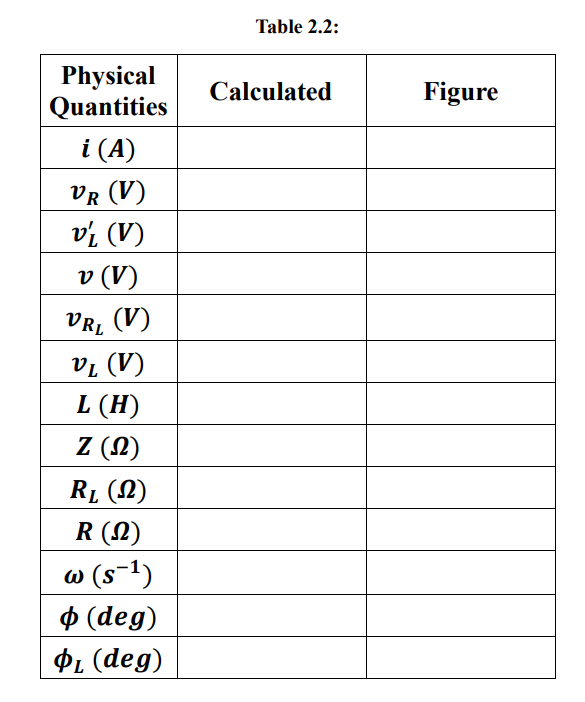
\includegraphics[width=0.9\linewidth]{path/to/your/image.png}
    \caption{Title of the Figure.}
    \label{fig:your_figure_label}
\end{figure}

\section{Discussion}
% Discuss the implications of your results, comparing them to theoretical predictions and literature.

\section{Conclusion}
% Summarize the main findings and their significance. Suggest any future work or improvements.

\section{Additional Resources}
The following resources can be reused for reference in future reports:
\begin{itemize}
    \item \textbf{Lab Manual:} Your Lab Manual Title, Year.
    \item \textbf{Online Resource:} Description and URL of a relevant online resource.
    \item \textbf{Book Reference:} Author, \textit{Title of the Book}, Publisher, Year.
\end{itemize}

\section{Bibliography}
The bibliography is consistent across all reports:
\begin{thebibliography}{9}
    \bibitem{lab_manual}
    ISTANBUL UNIVERSITY, 
    \textit{Physics Laboratory II Experiment Book: Electricity and Magnetism}, 
    Department of Physics, 2024.

    \bibitem{github}
    \textit{Source code and additional experiments are available in the GitHub repository.} \\ 
    Access it at: \url{https://github.com/ibeuler/LAB-Reports}

    % Add more bibliography entries as needed
\end{thebibliography}

\end{document}
